\documentclass{assignment}

\usepackage{float}
\usepackage{tikz}
\usepackage{adjustbox}
\usepackage{titlesec}
\usepackage{soul}
\usepackage{csvsimple}

\usepackage{bm}
\usepackage{amsmath,amssymb}

\usepackage{pgfplots}
\usepackage{graphics, epsfig}

\usepackage{graphicx}
\usepackage{subcaption}
\usepackage{matlab-prettifier}
\usepackage{multirow}

\usetikzlibrary{decorations.pathmorphing, decorations.markings}
\usetikzlibrary{positioning}

\usetikzlibrary{calc,patterns,angles,quotes}
\setlength{\parindent}{0pt}

\usetikzlibrary{shapes, arrows}
\tikzstyle{startstop} = [rectangle, rounded corners, minimum width=3cm, minimum height=1cm, text centered, draw=black, fill=red!30]
\tikzstyle{io} = [trapezium, trapezium stretches=true, trapezium left angle=70, trapezium right angle=110, minimum width=4cm, minimum height=1cm, text centered, draw=black, fill=blue!30]
\tikzstyle{process} = [rectangle, minimum width=4cm, minimum height=1cm, text centered, text width=4cm, draw=black, fill=orange!30]
\tikzstyle{decision} = [diamond, minimum width=3cm, minimum height=1cm, text centered, draw=black, fill=green!30]
\tikzstyle{arrow} = [thick,->,>=stealth]

\hypersetup{
pdftitle={Autonomous Vehicles},
pdfsubject={Assignment I},
pdfauthor={Tommaso Bocchietti}
}

\makeglossaries

\begin{document}

\title{Autonomous Vehicles \\ Assignment I: Use of ROS bags}
\author{Tommaso Bocchietti 10740309}
\date{A.Y. 2024/25}

\maketitle

\begin{figure}[H]
    \centering
    
\includegraphics[width=0.7\textwidth]{./pdf/Polimi_logo_coverpage.pdf}
    \label{fig:Polimi_logo}
\end{figure}

\clearpage
\tableofcontents
\listoffigures
% \listoftables
% \lstlistoflistings
% \printglossary[type=\acronymtype]

\clearpage
\section{Introduction}
\label{sec:introduction}

Motion planning is a fundamental aspect of autonomous vehicle navigation, enabling them to navigate complex environments while avoiding obstacles and reaching their destinations efficiently.

While in previous work we have focused on the implementation of two grid-based motion planning algorithms, namely Dijkstra and A*, this report aims to implement and analyze sampled-based motion planning algorithms.
Specifically, we focus on Rapidly-exploring Random Trees (RRT) and two of its variant, RRT* and a kinematically-learnt version of RRT.

After a brief introduction to the sampled-based motion planning approach, we present the implementation of the algorithms, followed by a discussion of the results obtained by running them on a set of predefined map scenarios.
An extensive comparison of the performance between the previously implemented A* algorithm and the RRT* algorithm is also reported, highlighting the strengths and weaknesses of each approach.

% Finally, just to demonstrate the capabilities of the implemented algorithms, we set up a simple control system for an 4-wheel steering-capable vehicle, and we show the ability of our RRT-kinematics algorithm to generate a trajectory that respect the non-holonomic constraints of the vehicle and safely navigate through a complex environment.

\paragraph{Report Structure}

The report is structured as follows:

\begin{itemize}
    \item In Section \ref{sec:sampling_based_planning}, we provide a brief introduction to the sampled-based motion planning algorithms, giving an overview of the single-query and multi-query approaches, and discussing the RRT algorithm and its variants.
    \item In Section \ref{sec:algorithm_implementation}, we present the all the three algorithms, RRT, RRT* and RRT-kinematics, explaining the main features of each one and the implementation details.
    \item In Section \ref{sec:algorithm_testing}, we present the results obtained by running the algorithms on a set of predefined map scenarios, and we discuss their performance in terms of computation time, path length and number of nodes sampled.
    \item In Section \ref{sec:grid_vs_sample_based_planning}, we compare the performance of the RRT* algorithm with the A* algorithm, highlighting the strengths and weaknesses of each approach.
          % \item In Section \ref{sec:autonomous_driving_demo}, we quickly introduce the simulated environment used to test the algorithms, and we show the ability of our RRT-kinematics algorithm to generate a trajectory that respect the non-holonomic constraints of the vehicle and safely navigate through a complex environment.
    \item In Section \ref{sec:conclusions}, we summarize the main findings of the report and discuss the future work that can be done to improve the algorithms and their performance.
\end{itemize}


\paragraph{Tools}

As for the tools used, \texttt{MATLAB} is employed as the main platform for implementing the algorithms and performing the analysis of the results.
% As for the simulation environment, we will use both \texttt{MATLAB}, \texttt{Simulink} and \texttt{ROS} to planning, control and visualize the vehicle behavior.
\section{Assignment Part A}
\label{sec:assignment_part_A}

In this section, we provide a brief overview of the requests associated with the first part of the assignment, along with a description of the approach taken to fulfill them.
Discussion of the results obtained is also included.



\subsection{Request}
\label{subsec:request_part_A}

Starting from the data collected in the provided \texttt{rosbag} file, the goal of this first part of assignment is to evalute at each time instant, the following quantities:

\begin{itemize}
    \item \textbf{Minimum distance} of the vehicle from the obstacles in the environment;
    \item \textbf{Estimate of \texttt{/cmd\_vel} command} sent to the vehicle during the simulation.
\end{itemize}

We also recal that the \texttt{rosbag} file was obtained by running a \texttt{Turtlebot3} robot of the model \texttt{burger} in a simulated environment, specifically the \texttt{turtlebot3\_world} provided by the \texttt{turtlebot3\_gazebo} package.

\begin{figure}[H]
    \centering
    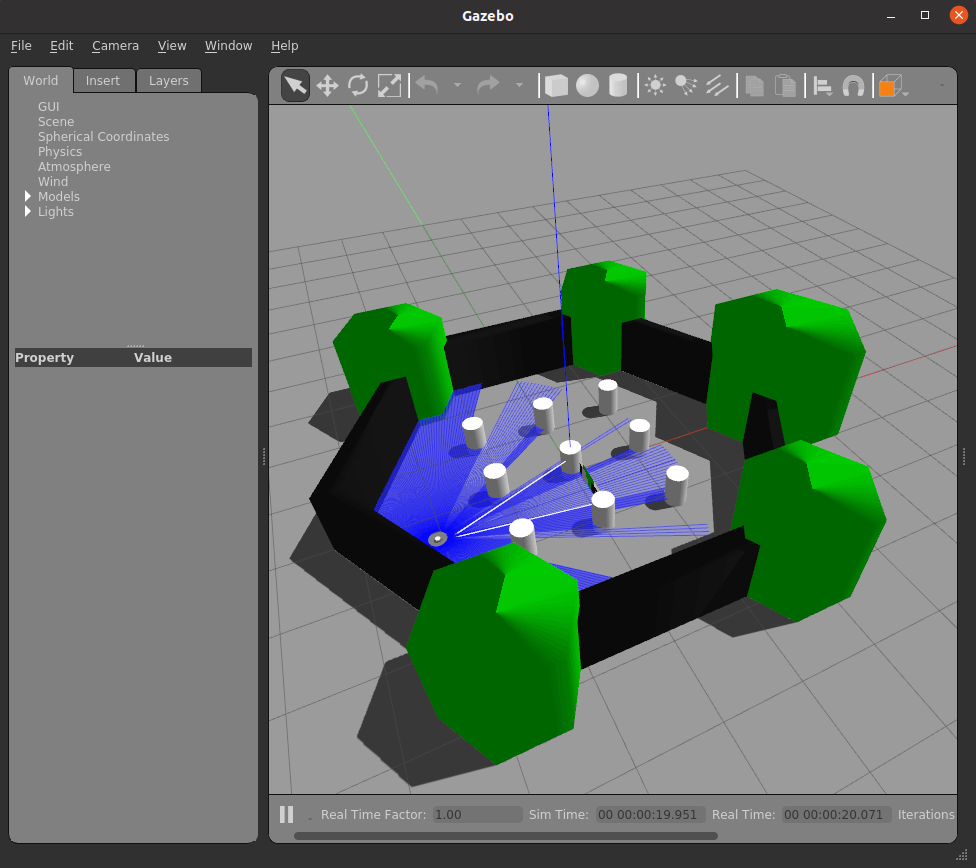
\includegraphics[width=0.6\textwidth]{./img/gazebo_world.png}
    \caption{Gazebo world used for the simulation. Credit to \url{https://emanual.robotis.com/}}
    \label{fig:turtlebot3_world}
\end{figure}



\subsection{Analysis}
\label{subsec:analysis_part_A}

At first, the \texttt{rosbag} file is loaded into \texttt{MATLAB} using the \texttt{rosbag} function, which allows to read and manipulate \texttt{rosbag} files in a convenient way.
A preliminary analysis of the data contained in the \texttt{rosbag} file is performed showing the following topics:

% \begin{lstlisting}[
%     style=Matlab-editor,
%     caption={Topics contained in the \texttt{rosbag} file.},
%     label={lst:rosbag_topics}
% ]
% bag = rosbag('bags/provided.bag');
% bag.AvailableTopics
% \end{lstlisting}

% Which returns the following topics:

\begin{table}[H]
    \centering
    \begin{tabular}{l|l|l}
        ~      & \textbf{NumMessages} & \textbf{MessageType}   \\
        \hline
        /clock & 110,710              & rosgraph\_msgs/Clock   \\
        /imu   & 110,240              & sensor\_msgs/Imu       \\
        /odom  & 3,316                & nav\_msgs/Odometry     \\
        /scan  & 552                  & sensor\_msgs/LaserScan \\
        /tf    & 3,316                & tf2\_msgs/TFMessage    \\
        \hline
    \end{tabular}
    \caption{Topics contained in the \texttt{rosbag} file.}
    \label{tab:rosbag_topics}
\end{table}


\subsubsection{Minimum distance from obstacles}
\label{subsubsec:minimum_distance}

Given the presence of the \texttt{/scan} topic, which contains the laser scan data, we can use it to compute the minimum distance from obstacles in the environment.
The \texttt{scan} message contains a field called \texttt{ranges}, which is an array of distances measured by the laser scanner at different angles.
The minimum distance can be computed by taking the minimum value of this array, which represents the closest obstacle detected by the laser scanner at that time instant.
The following code snippet shows how to extract the \texttt{ranges} field from the \texttt{/scan} topic and compute the minimum distance at each time instant:

\begin{lstlisting}[
    style=Matlab-editor,
    caption={Extracting the \texttt{ranges} field from the \texttt{/scan} topic and computing the minimum distance at each time step.},
    label={lst:minimum_distance}
]
scan = select(bag, 'Topic', '/scan');
scan_msgs = readMessages(scan, 'DataFormat', 'struct');
scan_time = scan.MessageList.Time - scan.StartTime;
scan_ranges = cell2mat(cellfun(@(msg) msg.Ranges(:)', scan_msgs, 'UniformOutput', false));
min(scan_ranges, [], 2)
\end{lstlisting}

One can also plot the minimum distance over time, as shown in Figure \ref{fig:minimum_distance}.

\begin{figure}[H]
    \centering
    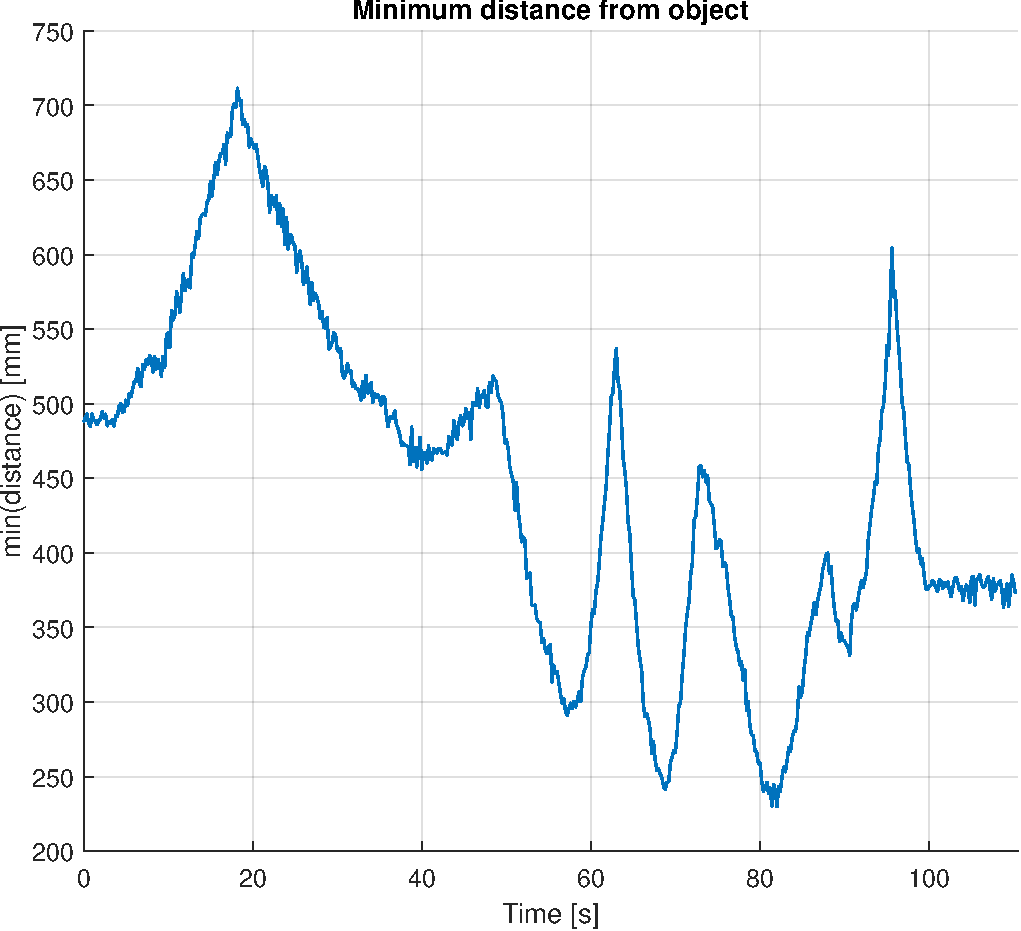
\includegraphics[width=0.7\textwidth]{./img/MATLAB/minimum_distance.pdf}
    \caption{Minimum distance from obstacles over time.}
    \label{fig:minimum_distance}
\end{figure}

It's important to notice that, being the data coming from a simulated environment, we can expect the accuracy of the laser scanner to be almost perfect (unless the simulation environment add noise on purpose), while on a real vehicle we could face issues like sensor noise or hit of minimum and/or maximum range of the laser scanner.
This could lead to a less accurate estimation of the minimum distance from obstacles, which could be a problem for the robot navigation and obstacle avoidance.


\subsubsection{Estimate of \texttt{/cmd\_vel} command}
\label{subsubsec:cmd_vel}

The \texttt{/cmd\_vel} topic usually contains the velocity commands sent to the robot, which are typically represented as linear and angular velocities.

As an exercise, given that in the provided \texttt{rosbag} file the \texttt{/cmd\_vel} topic has been removed, we can estimate the linear and angular velocities of the robot using the \texttt{/odom} topic, which contains the odometry data.
The \texttt{odom} message contains the position and orientation of the robot in the world frame, as measured by the odometry system.

Again, with a similar faschion as done for the \texttt{/scan} topic, we can extract the information from the \texttt{/odom} topic, save them in a matrix form and plot them.

\begin{figure}[H]
    \centering
    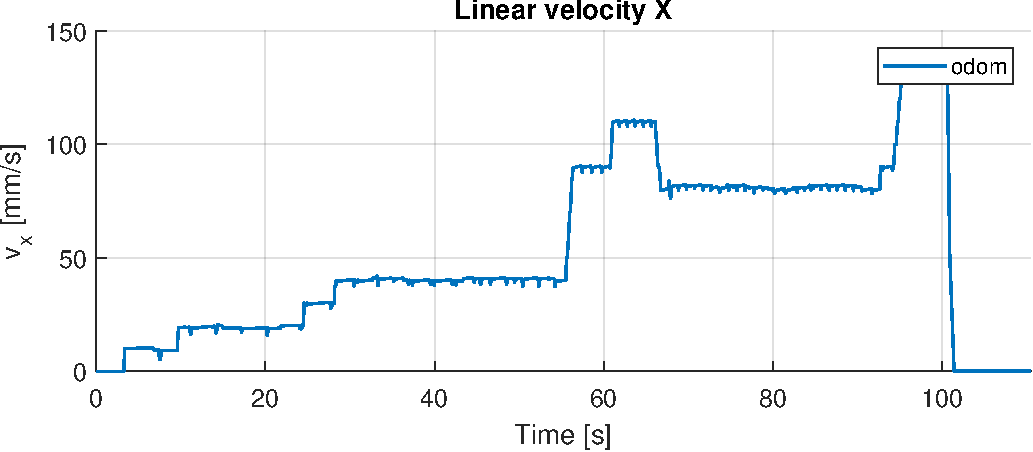
\includegraphics[width=0.8\textwidth]{./img/MATLAB/linear_velocity.pdf}
    \vspace{9pt}
    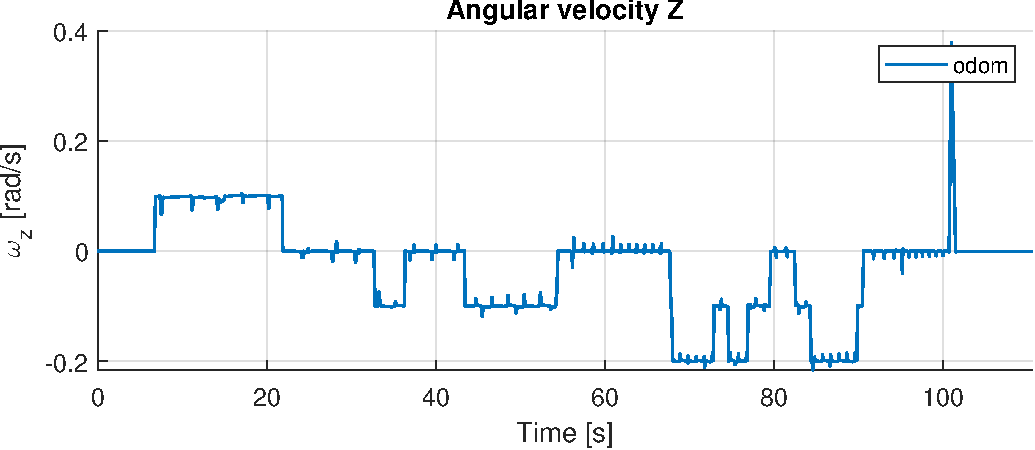
\includegraphics[width=0.8\textwidth]{./img/MATLAB/angular_velocity.pdf}
    \caption{Velocities of the robot over time, purerly based on the odometry data.}
    \label{fig:odom_velocities}
\end{figure}

Notice that one could have also possibly used the \texttt{/imu} topic to estimate both position and velocities of the robot (via single and double integration of the acceleration data).
However, due to the presence of noise in the IMU data and cumulative errors due to integration, this approach is definitely not recommended as it easily results in drifted output estimation.

On the other hand, a sensor fusion approach based for example on the Kalman filter could have been used to combine the two sources of data (IMU and odometry) ultimately increasing the overall accuracy.


\section{Assignment Part B}
\label{sec:assignment_part_B}

In this section, we provide a brief overview of the requests associated with the second part of the assignment, along with a description of the approach taken to fulfill them.
Discussion of the results obtained is also included in the following sections.


\subsection{Request}
\label{subsec:request_part_B}

Given that in the previous section we have estimated the control commands sent to the robot during the original simulation, in this second part we are asked to evaluate the accuracy of such commands.



\subsection{Analysis}
\label{subsec:analysis_part_B}

In order to evaluate the accuracy of the control commands sent to the robot during the simulation, we need to rerun a simulation by our own, using the same world and the same robot model, and then compare both the trajectory and the velocities with the ones saved in the original \texttt{rosbag} file.

We recall that our working environment is setup so that \texttt{ROS1} is running in the \texttt{WSL2} (Windows Subsystem for Linux) environment, specifically in \texttt{Ubuntu 20.04}, while \texttt{MATLAB 2024a} is running in Windows 10.
Based on these considerations, we can run the simulation in at least three different ways:

\begin{itemize}
    \item Create a publisher script in \texttt{MATLAB} that sends the commands to \texttt{ROS1} running in \texttt{WSL2};
    \item Create a publisher in \texttt{Simulink} that sends the commands to \texttt{ROS1} running in \texttt{WSL2};
    \item Perform the analysis directly in \texttt{WSL2} using the native commands of \texttt{rosbag} to automatically replay the estimated commands.
\end{itemize}

At first, we tried to create a publisher script in \texttt{MATLAB} that was sending the commands over the bridged network, pacing the sender based on the original timing of the \texttt{/odom} topic.
However, we encountered some major issues with the timing of the commands, which were sent at almost unpredictable intervals, leading to a completely different behavior of the robot in the simulation.

In order to avoid or at least reduce the issues related to the timing of the commands, we decided to directly move to the third option, which is to perform the analysis directly in \texttt{WSL2} using the native commands of \texttt{rosbag} to automatically replay the estimated commands.
At first, the \texttt{/odom} topic has been ported to a new \texttt{rosbag} file using a simple \texttt{python} script, which is able to read the original \texttt{rosbag} file and write the \texttt{/odom} topic to a new \texttt{rosbag} file while also reshaping the data to match the type of the \texttt{/cmd\_vel} topic.
In particular, the following relationship table has been implemented:

\begin{table}[H]
    \centering
    \begin{tabular}{c|c}
        \textbf{/odom}            & \textbf{/cmd\_vel} \\
        \hline
        msg.Twist.Twist.Linear.X  & msg.Linear.X       \\
        msg.Twist.Twist.Angular.Z & msg.Angular.Z      \\
        \hline
    \end{tabular}
    \caption{Relationship between the \texttt{/odom} and \texttt{/cmd\_vel} topics.}
    \label{tab:rosbag_relationship}
\end{table}

Once the content of the \texttt{/odom} topic has been saved as \texttt{/cmd\_vel} topic in a new \texttt{rosbag} file, we can use the \texttt{rosbag play} command to replay the commands in the simulation.

In Figure \ref{fig:trajectory_comparison} we can see the comparison of the trajectories performed by the original simulation and the one performed by the replayed commands.

\begin{figure}[H]
    \centering
    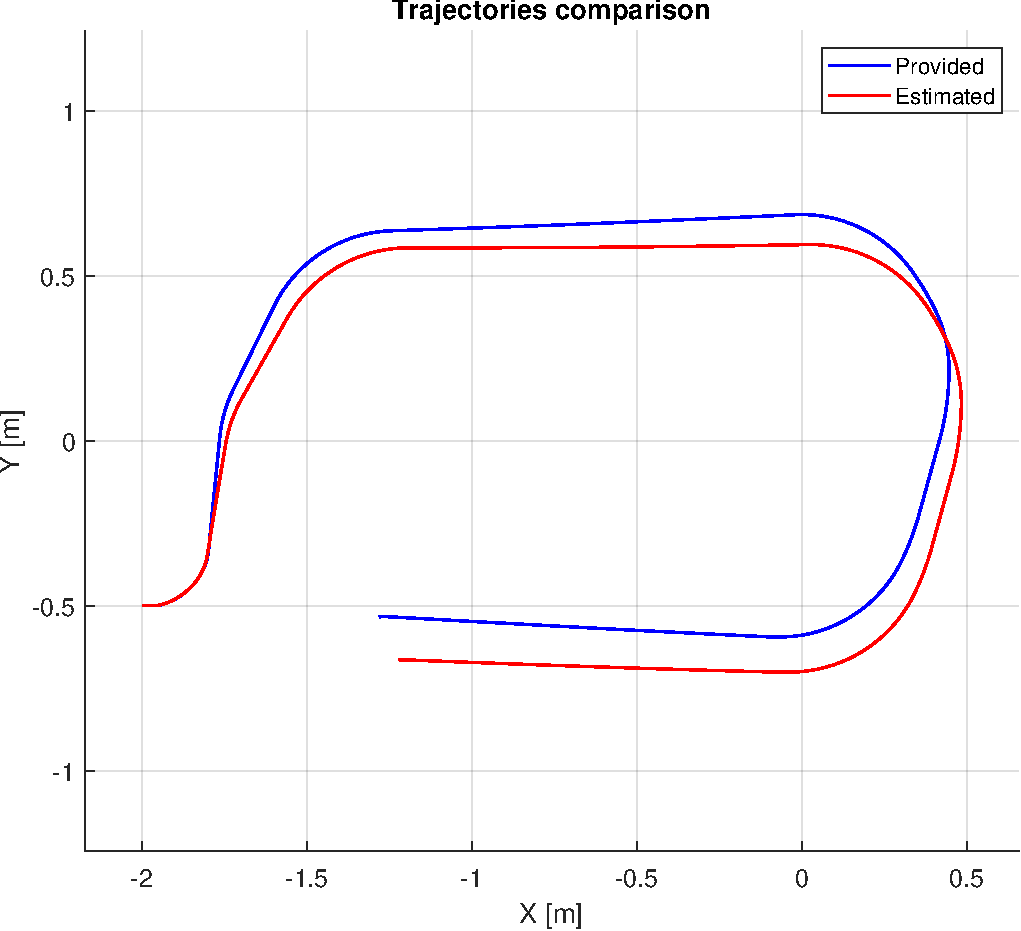
\includegraphics[width=0.8\textwidth]{./img/MATLAB/trajectories_comparison.pdf}
    \caption{Comparison of the trajectories performed by the original simulation and the one performed by the replayed commands.}
    \label{fig:trajectory_comparison}
\end{figure}

One can clearly see that the two trajectories are not completely overlapping.

Looking at the values of the actual velocities of the robot during the simulation, we can see a minor discrepancy between the original simulation and the one performed by the replayed commands, similarly to the behaviour observer for the trajectories.
Figure \ref{fig:velocity_comparison} shows the comparison of the velocities performed by the original simulation and the one performed by the replayed commands.

\begin{figure}[H]
    \centering
    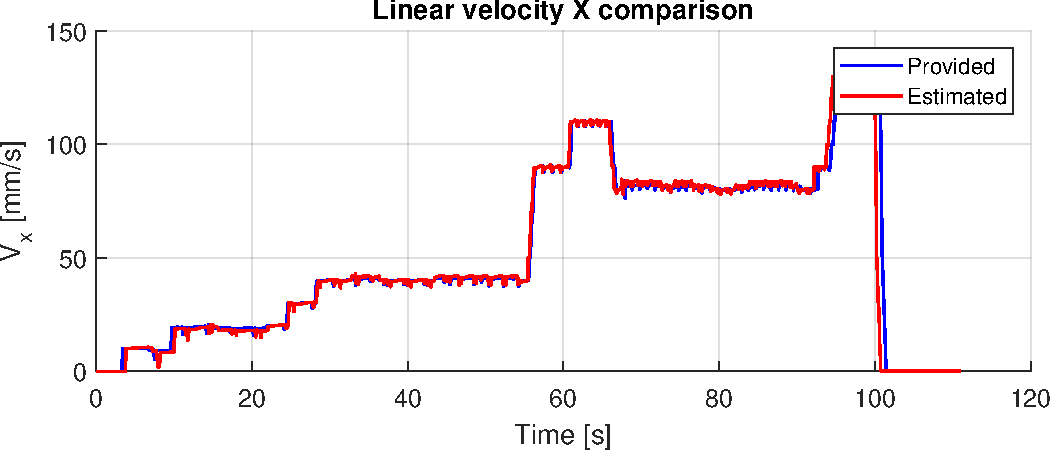
\includegraphics[width=0.8\textwidth]{./img/MATLAB/linear_velocity_comparison.pdf}

    \vspace{10pt}

    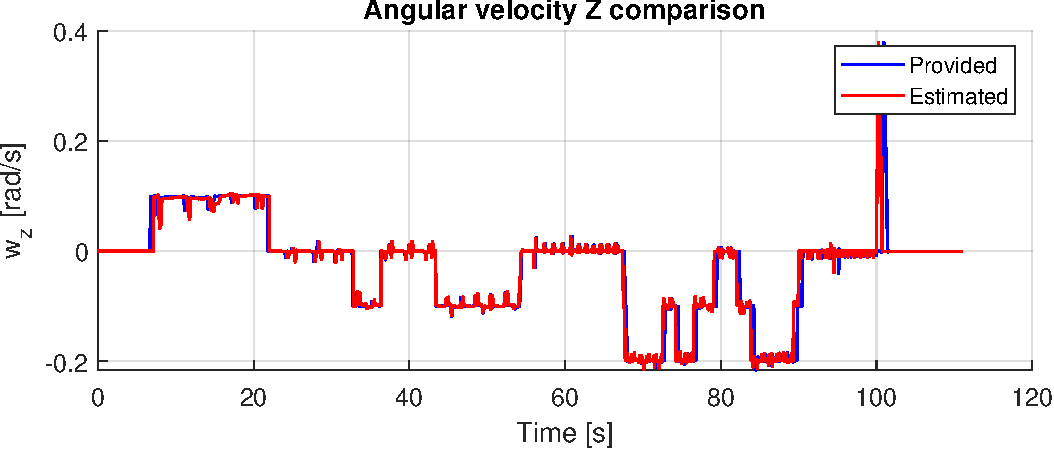
\includegraphics[width=0.8\textwidth]{./img/MATLAB/angular_velocity_comparison.pdf}
    \caption{Comparison of the velocities performed by the original simulation and the one performed by the replayed commands.}
    \label{fig:velocity_comparison}
\end{figure}

Again, some minor issues related to timing can be observed.
For some reason that the author is not able to determine, the \texttt{rosbag play} command is not able to replay the commands at the exact same pace as the original simulation, leading to a slight shift in the velocities.

What is also interesting to notice, are the juggling of the velocities along the whole simulation.
These are, in fact, not desired behaviors and most probably caused by the simulated environment itself.
\section{Conclusions}
\label{sec:conclusions}

In this short report, we have presented the results of the fifth assignment of the course on Autonomous Vehicles.
We have briefly explained what FSMs are and how they can be used to model the behavior of generic systems.

We have also presented a possible FMSs implementation about a car parking system, which is able to coordinate the behavior of the car and the parking gate.
The results presented have shown the effectiveness of the proposed solution.

The current solution could be improved under many aspects.
For example, one could think of implementing features like error handling, or ticket authentication and validation, or even a more complex parking system composed of multiple parking gates and cars that must coordinated over the network.

We believe that FMSs are a power tool that can often replace traditional programming paradigms, allowing to model complex systems in a more intuitive way.
Further studies on this topic could be useful to understand the full potential of FMSs and their applications in the field of autonomous vehicles and robotics in general.

\vspace*{\fill}
\nocite{*}
\bibliographystyle{plain}
\bibliography{references.bib}

\end{document}
